\documentclass[aspectratio=169,11pt]{beamer}

% ============================================================
% Theme
% ============================================================
\usetheme{Madrid}
\usecolortheme{seahorse}
\setbeamertemplate{navigation symbols}{}


% ============================================================
% Encoding
% ============================================================
\usepackage[utf8]{inputenc}
\usepackage[T1]{fontenc}
\usepackage{lmodern}

% ============================================================
% Packages
% ============================================================
\usepackage{amsmath,amssymb}
\usepackage{xcolor}
\usepackage{booktabs}
\usepackage{array}
\usepackage{listings}
\usepackage{tikz}
\usetikzlibrary{arrows.meta,positioning,calc,fit}
\usepackage{hyperref}
\hypersetup{pdfpagemode=UseNone}

% ============================================================
% Custom Colors
% ============================================================
\definecolor{deepblue}{RGB}{0,51,102}
\definecolor{softblue}{RGB}{220,235,247}
\definecolor{softred}{RGB}{250,224,224}
\definecolor{codebg}{RGB}{248,248,248}

% ============================================================
% Beamer Colors
% ============================================================
\setbeamercolor{structure}{fg=deepblue}
\setbeamercolor{frametitle}{fg=white,bg=deepblue}
\setbeamercolor{block title}{fg=white,bg=deepblue}
\setbeamercolor{block body}{fg=black,bg=softblue}
\setbeamercolor{alertblock title}{fg=white,bg=red!70!black}
\setbeamercolor{alertblock body}{fg=black,bg=softred}

% ============================================================
% Listings
% ============================================================
\lstset{
	basicstyle=\ttfamily\small,
	backgroundcolor=\color{codebg},
	frame=single,
	breaklines=true,
	columns=fullflexible,
	showstringspaces=false,
	keywordstyle=\color{blue}\bfseries,
	commentstyle=\color{gray},
	stringstyle=\color{red}
}

% ============================================================
% Title
% ============================================================
% ============================================================
% Title
% ============================================================
\title{Concurrency \& Distributed Systems}
\subtitle{Week 3: Deadlocks, Inspection, and Prevention}
\author{Dr. Mohamad Aoude}
\institute{Lebanese University \\ Faculty of Engineering}
\date{}

% ============================================================
% TikZ Styles
% ============================================================
\tikzset{
	box/.style={draw, rounded corners=2pt, align=center, inner sep=6pt},
	smallbox/.style={draw, rounded corners=2pt, align=center, inner sep=3pt},
	arrow/.style={-Latex, line width=0.8pt},
	dashedarrow/.style={-Latex, dashed, line width=0.8pt},
	tinylabel/.style={font=\scriptsize},
	pill/.style={draw, rounded corners=10pt, inner sep=4pt, align=center}
}

\begin{document}
		% ============================================================
	\begin{frame}
		\titlepage
	\end{frame}
	% ============================================================
	% Block 4 --- Inspecting Deadlock
	% ============================================================
	
	\begin{frame}{Block 4 --- Inspecting Deadlock}
		\begin{block}{Goal}
			Move from theory to diagnosis.
		\end{block}
		
		\bigskip
		
		Students should learn how to:
		\begin{itemize}
			\item identify BLOCKED threads
			\item identify lock ownership
			\item reconstruct circular wait from evidence
		\end{itemize}
		
		\bigskip
		
		\begin{alertblock}{Engineering mindset}
			A deadlock is not only a concept.  
			It is something you must be able to detect in a running system.
		\end{alertblock}
	\end{frame}
	
	% ============================================================
	\begin{frame}[fragile]{Inspecting Deadlock with \texttt{jstack}}
		\begin{lstlisting}[language=bash]
			jps
			jstack -l <PID>
		\end{lstlisting}
		
		\vspace{0.3cm}
		
		\begin{block}{Workflow}
			\begin{enumerate}
				\item Use \texttt{jps} to find the Java process ID
				\item Use \texttt{jstack -l} to dump all thread stacks
				\item Search for blocked threads and monitor ownership
				\item Reconstruct the waiting graph from the dump
			\end{enumerate}
		\end{block}
		
		\begin{alertblock}{Live-debugging mindset}
			Production is hung. CPU is low. No errors.  
			You SSH in, run \texttt{jstack}, and start reading the system like evidence.
		\end{alertblock}
	\end{frame}
	
	% ============================================================
	\begin{frame}[fragile]{Normal Contention vs Deadlocked Dump}
		\begin{columns}[T]
			\begin{column}{0.47\textwidth}
				\begin{block}{Normal contention}
					\begin{lstlisting}[language=Java]
"Worker-1" ...
- locked <0x1001>
						
"Worker-2" ...
- waiting to lock <0x1001>
					\end{lstlisting}
				\end{block}
			\end{column}
			\begin{column}{0.47\textwidth}
				\begin{block}{Deadlock}
					\begin{lstlisting}[language=Java]
"Worker-1" ...
- locked <0x1001>
- waiting to lock <0x2002>
						
"Worker-2" ...
- locked <0x2002>
- waiting to lock <0x1001>
					\end{lstlisting}
				\end{block}
			\end{column}
		\end{columns}
		
		\vspace{0.3cm}
		\begin{alertblock}{Key distinction}
			Two blocked threads on one lock may be healthy contention.  
			Deadlock requires a \textbf{cycle}.
		\end{alertblock}
	\end{frame}
	
	% ============================================================
	\begin{frame}[fragile]{What Students Should Look For in a Thread Dump}
		\begin{lstlisting}[language=Java]
			"Thread-1" ...
			- waiting to lock <0x00000007d5c8>
			- locked <0x00000007d5b8>
			
			"Thread-2" ...
			- waiting to lock <0x00000007d5b8>
			- locked <0x00000007d5c8>
		\end{lstlisting}
		
		\vspace{0.3cm}
		
		\begin{alertblock}{Interpretation}
			Thread 1 holds one monitor and waits for the other.  
			Thread 2 holds the other monitor and waits for the first.
		\end{alertblock}
		
		\vspace{0.2cm}
		\centering
		\begin{tabular}{@{}lll@{}}
			\toprule
			\textbf{State} & \textbf{Meaning} & \textbf{Deadlock relevance} \\
			\midrule
			BLOCKED & waiting for monitor entry & direct indicator \\
			WAITING & waiting for notify/join & may be unrelated \\
			TIMED\_WAITING & sleeping/timeout wait & often benign \\
			\bottomrule
		\end{tabular}
	\end{frame}
	
	% ============================================================
	\begin{frame}{How Monitor Addresses Reveal the Cycle}
		\begin{block}{Key idea}
			The hexadecimal monitor addresses are the evidence trail.
		\end{block}
		
		\bigskip
		
		\begin{itemize}
			\item \texttt{locked <0x...>} tells you what the thread owns
			\item \texttt{waiting to lock <0x...>} tells you what it needs
			\item Matching these addresses across threads reveals the dependency cycle
		\end{itemize}
		
		\bigskip
		
		\begin{alertblock}{False-positive warning}
			Two threads blocked on the same lock do \textbf{not} automatically mean deadlock.  
			Look for a closed cycle of ownership and waiting.
		\end{alertblock}
	\end{frame}
	
	% ============================================================
	\begin{frame}{Thread Dump Reasoning Pattern}
		\centering
		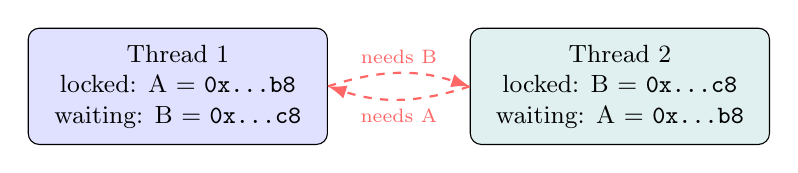
\begin{tikzpicture}[
			node distance=12mm and 18mm,
			stepbox/.style={draw, rounded corners=4pt, align=center, inner sep=6pt, font=\small}
			]
			\node[stepbox, fill=blue!12, minimum width=3.8cm] (t1)
			{Thread 1\\locked: A = \texttt{0x...b8}\\waiting: B = \texttt{0x...c8}};
			
			\node[stepbox, fill=teal!12, right=of t1, minimum width=3.8cm] (t2)
			{Thread 2\\locked: B = \texttt{0x...c8}\\waiting: A = \texttt{0x...b8}};
			
			\draw[dashedarrow, red!60] (t1.east) to[bend left=18] node[above, font=\scriptsize]{needs B} (t2.west);
			\draw[dashedarrow, red!60] (t2.west) to[bend left=18] node[below, font=\scriptsize]{needs A} (t1.east);
		\end{tikzpicture}
		
		\vspace{0.4cm}
		
		\begin{block}{Pattern}
			Read the dump as a graph:
			\[
			\text{thread} \rightarrow \text{holds lock} \rightarrow \text{waits for other lock}
			\]
			If the graph closes back on itself, you have deadlock.
		\end{block}
	\end{frame}
	
	% ============================================================
	\begin{frame}[fragile]{Mini-Challenge --- Read the Dump}
		\begin{lstlisting}[language=Java]
			"Worker-A" ...
			- locked <0x1001>
			- waiting to lock <0x2002>
			
			"Worker-B" ...
			- locked <0x2002>
			- waiting to lock <0x3003>
			
			"Worker-C" ...
			- locked <0x3003>
			- waiting to lock <0x1001>
		\end{lstlisting}
		
		\vspace{0.3cm}
		
		\begin{alertblock}{Question}
			Is this a deadlock? How many threads are involved?  
			Draw the cycle.
		\end{alertblock}
	\end{frame}
	
	% ============================================================
	\begin{frame}{Inspecting Deadlock with VisualVM}
		\begin{block}{Visual cues matter}
			VisualVM lets students \textbf{see} the deadlock, not only read about it.
		\end{block}
		
		\bigskip
		
		Use:
		\begin{itemize}
			\item the \textbf{Threads} tab
			\item the thread states view
			\item the deadlock detection feature
		\end{itemize}
		
		\bigskip
		
		\begin{alertblock}{Psychological impact}
			When students see the tool reveal the bug automatically,
			deadlock stops being abstract and becomes real.
		\end{alertblock}
		
		\vspace{0.2cm}
		{\scriptsize Placeholder for class version: insert annotated screenshot of VisualVM deadlock view.}
	\end{frame}
	
	% ============================================================
	\begin{frame}{Why Tooling Matters}
		\begin{itemize}
			\item Theory explains why deadlock occurs
			\item Tools reveal where it occurs
			\item Thread dumps translate runtime behavior into analyzable evidence
		\end{itemize}
		
		\bigskip
		
		\begin{block}{Engineering lesson}
			A strong engineer does not stop at “I know deadlock.”  
			A strong engineer can also diagnose it in a live or failing system.
		\end{block}
		
		\bigskip
		
		\begin{alertblock}{Forward-looking note}
			Programmatic inspection is also possible with \texttt{ThreadMXBean.findDeadlockedThreads()}.
		\end{alertblock}
	\end{frame}
	
	% ============================================================
	\begin{frame}[fragile]{Programmatic Deadlock Detection Preview}
		\begin{lstlisting}[language=Java]
			ThreadMXBean bean = ManagementFactory.getThreadMXBean();
			long[] ids = bean.findDeadlockedThreads();
			
			if (ids != null) {
				System.out.println("Deadlock detected");
			}
		\end{lstlisting}
		
		\vspace{0.3cm}
		\begin{block}{Why this matters}
			Manual inspection is essential for learning.  
			Programmatic detection is essential for monitoring and observability.
		\end{block}
	\end{frame}
	
	% ============================================================
	% Block 5 --- Reducing Lock Risk
	% ============================================================
	
	\begin{frame}{Block 5 --- Reducing Lock Risk}
		\begin{block}{Goal}
			Not every lock causes deadlock, but poor lock design increases risk.
		\end{block}
		
		\bigskip
		
		Practical strategies:
		\begin{enumerate}
			\item Keep critical sections small
			\item Avoid nested locks when possible
			\item Use global lock ordering
			\item Avoid long blocking operations inside \texttt{synchronized}
		\end{enumerate}
	\end{frame}
	
	% ============================================================
	\begin{frame}[fragile]{Strategy 1 --- Keep Critical Sections Small}
		\begin{columns}[T]
			\begin{column}{0.47\textwidth}
				\begin{block}{Too broad}
					\begin{lstlisting}[language=Java]
synchronized(account) {
	complexCalculation();
	Thread.sleep(100);
	databaseCall();
	account.update();
}
					\end{lstlisting}
				\end{block}
			\end{column}
			\begin{column}{0.47\textwidth}
				\begin{block}{Better}
					\begin{lstlisting}[language=Java]
complexCalculation();
databaseCall();
						
synchronized(account) {
	account.update();
}
					\end{lstlisting}
				\end{block}
			\end{column}
		\end{columns}
		
		\vspace{0.2cm}
		\begin{alertblock}{Rule of thumb}
			Lock the shared state, not the entire workflow.
		\end{alertblock}
	\end{frame}
	
	% ============================================================
	\begin{frame}{Strategy 2 --- Avoid Nested Locks When Possible}
		\begin{block}{Meaning}
			Every additional lock increases structural risk.
		\end{block}
		
		\bigskip
		
		\begin{itemize}
			\item One lock can create contention
			\item Two or more locks can create dependency cycles
			\item Nested locking should be treated as a design decision, not a casual habit
		\end{itemize}
		
		\bigskip
		
		\begin{alertblock}{Practical lesson}
			If one lock is enough, do not introduce two.
		\end{alertblock}
	\end{frame}
	
	% ============================================================
	\begin{frame}{Strategy 3 --- Use Global Lock Ordering}
		\begin{block}{Meaning}
			If multiple locks must be acquired, all threads should acquire them in the same order.
		\end{block}
		
		\bigskip
		
		\begin{itemize}
			\item This prevents circular wait
			\item This is the cleanest structural deadlock-prevention strategy
			\item It scales from simple demos to real systems
		\end{itemize}
		
		\bigskip
		
		\begin{alertblock}{Dynamic-resource teaser}
			If locks are chosen at runtime, order them by a stable rule:
			account ID, canonical key, or another immutable criterion.
		\end{alertblock}
	\end{frame}
	
	% ============================================================
	\begin{frame}{Strategy 4 --- Avoid Long Blocking Operations Inside \texttt{synchronized}}
		\begin{block}{Examples of risky work inside a lock}
			\begin{itemize}
				\item sleeping
				\item network I/O
				\item file I/O
				\item database calls
				\item waiting for user input
			\end{itemize}
		\end{block}
		
		\bigskip
		
		\begin{alertblock}{Why dangerous?}
			The longer a thread holds a lock, the longer other threads wait,
			and the higher the contention and deadlock risk.
		\end{alertblock}
	\end{frame}
	
	% ============================================================
	\begin{frame}{Common Anti-Patterns That Increase Deadlock Risk}
		\begin{itemize}
			\item calling external callbacks while holding a lock
			\item starting a thread inside a synchronized region
			\item performing long I/O under a monitor
			\item mixing multiple locks without a documented order
		\end{itemize}
		
		\bigskip
		
		\begin{block}{Engineering interpretation}
			Deadlock often appears not from one line, but from poor interaction between local design choices.
		\end{block}
	\end{frame}
	
	% ============================================================
	\begin{frame}{Lock Granularity Spectrum}
		\centering
		\begin{tabular}{@{}lll@{}}
			\toprule
			\textbf{Granularity} & \textbf{Advantage} & \textbf{Cost} \\
			\midrule
			Coarse-grained & simple reasoning & lower concurrency \\
			Medium & balanced trade-off & moderate complexity \\
			Fine-grained & higher concurrency & higher deadlock/comprehension risk \\
			\bottomrule
		\end{tabular}
		
		\bigskip
		
		\begin{alertblock}{Lesson}
			More concurrency often means more reasoning complexity.
		\end{alertblock}
	\end{frame}
	
	% ============================================================
	\begin{frame}{Performance vs Correctness}
		\begin{block}{Important trade-off}
			Locks improve correctness, but excessive locking can reduce concurrency.
		\end{block}
		
		\bigskip
		
		\begin{itemize}
			\item Too little locking \(\Rightarrow\) races and incorrect results
			\item Too much locking \(\Rightarrow\) contention, blocking, and deadlock risk
		\end{itemize}
		
		\bigskip
		
		\begin{alertblock}{Engineering balance}
			The goal is not “more locks.”  
			The goal is \textbf{correct locking with minimal necessary blocking}.
		\end{alertblock}
	\end{frame}
	
	% ============================================================
	\begin{frame}{Design Mindset for Safer Locking}
		\begin{enumerate}
			\item Ask what shared state actually needs protection
			\item Minimize the scope and duration of the lock
			\item Check whether multiple locks are really necessary
			\item Enforce a global order whenever multiple locks exist
		\end{enumerate}
		
		\bigskip
		
		\begin{block}{Mindset}
			Do not treat synchronization as decoration.  
			Treat it as a structural part of system design.
		\end{block}
	\end{frame}
	
	% ============================================================
	% End-of-week conceptual summary
	% ============================================================
	
	\begin{frame}{Week 3 Knowledge Check}
		\begin{enumerate}
			\item What is the difference between a race condition and a deadlock?
			\item If a thread is \texttt{BLOCKED}, is it always deadlocked?
			\item Which Coffman condition does lock ordering eliminate?
			\item Does \texttt{synchronized} help only with exclusion, or also with visibility?
		\end{enumerate}
		
		\bigskip
		
		\begin{alertblock}{Purpose}
			Before moving forward, students should connect safety, visibility, and liveness into one mental model.
		\end{alertblock}
	\end{frame}
	
	% ============================================================
	\begin{frame}{End-of-Week Conceptual Summary}
		Students now understand:
		
		\begin{itemize}
			\item what a monitor is
			\item what mutual exclusion is
			\item what visibility means
			\item what happens-before guarantees
			\item how synchronization eliminates races
			\item how deadlock occurs
			\item how to prevent deadlock
			\item how to inspect blocked threads
		\end{itemize}
	\end{frame}
	
	% ============================================================
	\begin{frame}{What Changed This Week?}
		\begin{block}{At the start}
			Students knew threads can run concurrently.
		\end{block}
		
		\bigskip
		
		\begin{block}{At the end}
			Students now understand that concurrency requires:
			\begin{itemize}
				\item control of shared-state access
				\item memory visibility guarantees
				\item liveness-aware lock design
				\item practical debugging of blocked systems
			\end{itemize}
		\end{block}
	\end{frame}
	
	% ============================================================
	% Bridge to Week 4
	% ============================================================
	
	\begin{frame}{Bridge to Week 4}
		\begin{alertblock}{Key question}
			Is locking the only way to ensure correctness?
		\end{alertblock}
		
		\bigskip
		
		Preview:
		\begin{itemize}
			\item \texttt{AtomicInteger}
			\item hardware Compare-And-Swap (CAS)
			\item lock-free programming
			\item performance and contention
		\end{itemize}
		
		\bigskip
		
		\begin{block}{Concrete contrast}
			With locks, threads often queue and wait.  
			With atomic operations, threads may retry without blocking.
		\end{block}
	\end{frame}
	
	% ============================================================
	\begin{frame}{Week 4 --- Memory Visibility}
		Next week we go deeper into memory behavior itself:
		
		\begin{itemize}
			\item Java Memory Model
			\item \texttt{volatile}
			\item happens-before
			\item visibility vs atomicity
		\end{itemize}
		
		\bigskip
		
		\begin{block}{Recall prompt}
			\texttt{synchronized} guarantees visibility.  
			What if we need visibility, but not full mutual exclusion?
		\end{block}
		
		\vspace{0.2cm}
		
		\begin{block}{Lab preview}
			\begin{itemize}
				\item broken double-checked locking
				\item fixing it with \texttt{volatile}
				\item demonstrating stale reads
			\end{itemize}
		\end{block}
	\end{frame}
	
	% ============================================================
	\begin{frame}[fragile]{Week 4 Teaser --- Why \texttt{volatile} Matters}
		\begin{lstlisting}[language=Java]
			if (instance == null) {
				synchronized(lock) {
					if (instance == null) {
						instance = new Helper();
					}
				}
			}
		\end{lstlisting}
		
		\vspace{0.3cm}
		\begin{alertblock}{Question}
			What could go wrong here without \texttt{volatile}?  
			Think about visibility and instruction reordering.
		\end{alertblock}
	\end{frame}
	
	% ============================================================
	\begin{frame}{Final Exercise for the Week}
		\begin{block}{Take-home challenge}
			\begin{enumerate}
				\item Write a small Java program that deliberately deadlocks
				\item Use \texttt{jstack} to inspect it
				\item Reconstruct the dependency cycle
				\item Fix it with lock ordering
				\item Verify that the deadlock disappears
			\end{enumerate}
		\end{block}
		
		\bigskip
		
		\begin{alertblock}{Skill loop}
			Create \(\rightarrow\) detect \(\rightarrow\) explain \(\rightarrow\) prevent
		\end{alertblock}
	\end{frame}
	
	% ============================================================
	\begin{frame}{Final Thought for the Week}
		\begin{block}{Big idea}
			Concurrency is not only about making things run at the same time.
		\end{block}
		
		\bigskip
		
		It is about:
		\begin{itemize}
			\item controlling interference
			\item preserving correctness
			\item ensuring visibility
			\item maintaining progress
		\end{itemize}
		
		\bigskip
		
		\begin{alertblock}{Mantra}
			Concurrency is not about stopping threads from running.  
			It is about ensuring they run \textbf{correctly together}.
		\end{alertblock}
	\end{frame}
\end{document}